\section{问题三：扰流机理识别与聚类可分性分析}

\subsection{扰流特征构造与重要性分析}

扰流状态会改变圆管截面速度剖面，使不同声道对截面平均速度的代表性发生变化。Zhao 等的 CFD 研究表明，双弯管等复杂管路可产生强非对称与旋流剖面，声道方向会影响多路径流量计的积分误差；Papathanasiou 等进一步通过流动仿真说明，扰流入口条件下的声道布置和修正因子需要协同设计\cite{Zhao2014CFD,Papathanasiou2022FlowDC}。国内关于上游扰流和非充分发展流的研究也观察到扰流条件对计量准确度及不同声道响应的显著影响\cite{JinUpstreamDisturbance,SuUnderdevelopedFlow}。

Sakhavi 和 Nouri 的广义速度剖面研究说明，固定积分规则的精度依赖其假设的速度分布；当实际剖面偏离该假设时，需要利用多声道状态降低模型敏感性\cite{Sakhavi2022GeneralizedProfile}。剖面修正因子与在用误差补偿研究通常保留物理估计的主尺度，再对稳定系统残差进行标定\cite{Mousavi2020FPCF,Gryshanova2023CorrectionFactor,Li2023MLInUse}；这一思路为从多声道剖面特征解释扰流附加误差提供了依据。据此，本文构造自定义紧凑物理特征集（compact physical features）描述在线剖面状态，没有把人工扰流编号 \texttt{disturbance\_id} 作为模型输入。

为直观说明上述机理，图~\ref{fig:disturbance_profile_representativeness} 按附件 7 给定的五声道位置绘制剖面示意，并列出附件 1 中同一流量点下 D0 与 D3 窗口均值的代表性对比。彩色云图用于说明速度剖面由近似对称向偏斜状态变化。

\begin{figure}[!htbp]
  \centering
  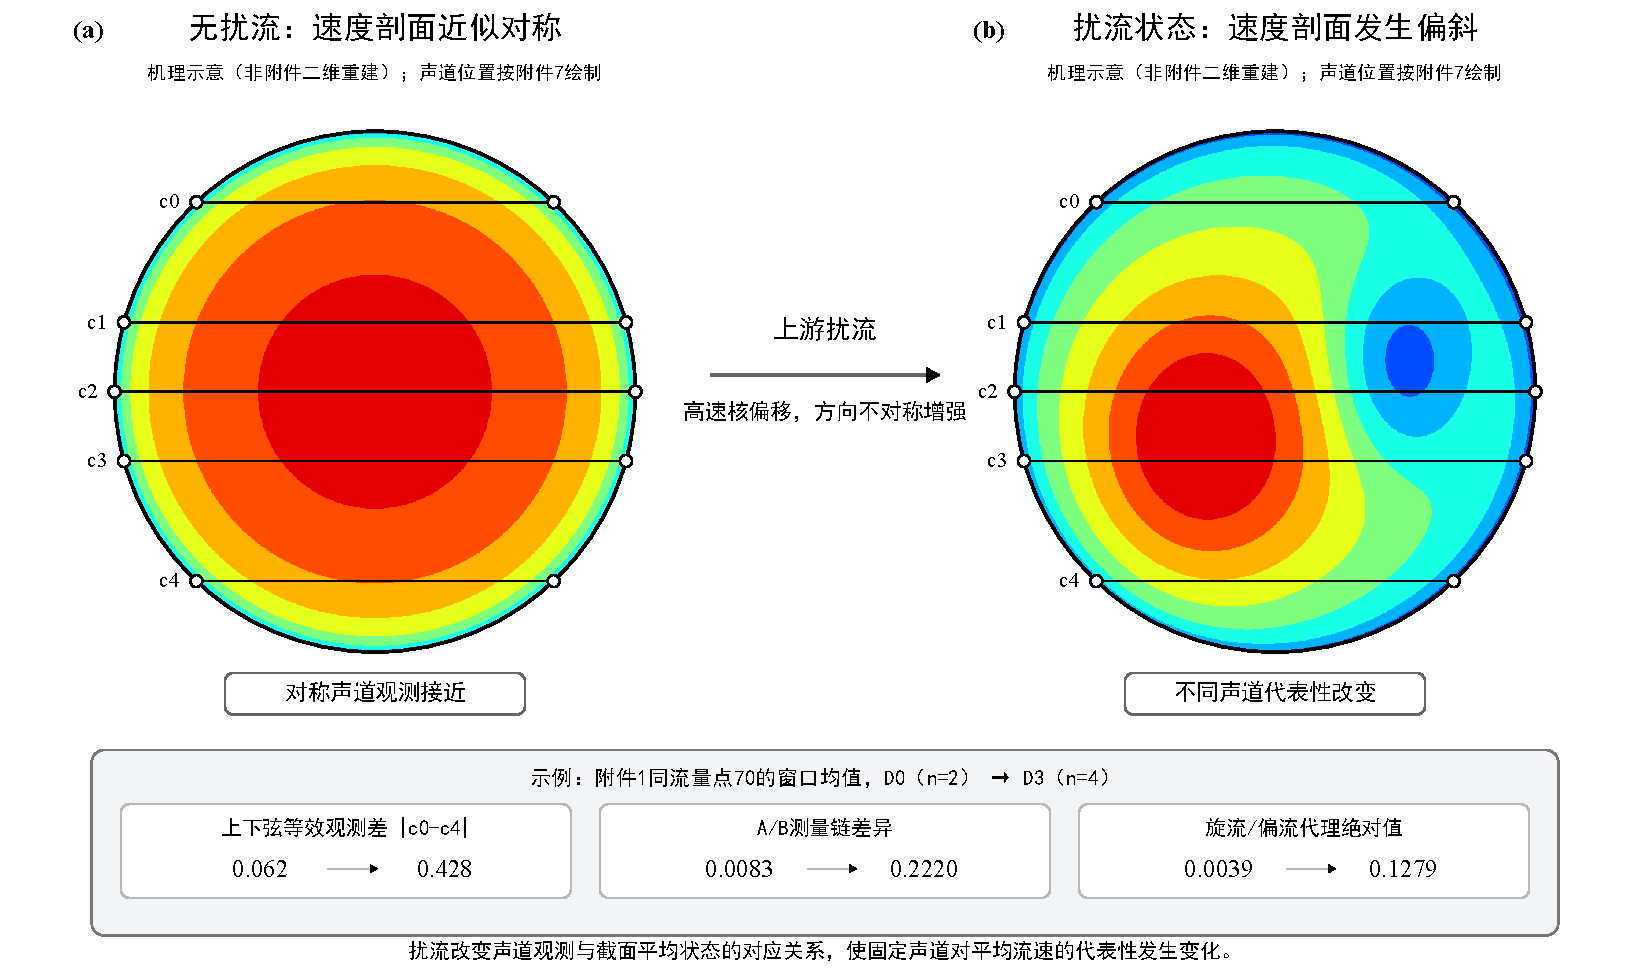
\includegraphics[width=0.98\textwidth]{../figures/fig_disturbance_profile_representativeness.pdf}
  \caption{扰流导致速度剖面偏斜及声道代表性变化示意}
  \label{fig:disturbance_profile_representativeness}
\end{figure}

流量尺度由 $q$ 和 $q^2$ 表示。剖面形态不再用单个声道概括，而是考察中心相对整体的偏离、边缘与内侧差异以及上下响应差。A/B 方向不对称和旋流分别由 \texttt{profile\_ab\_abs}、\texttt{profile\_swirl} 等变量描述。动态与零点变量只保留少量稳定性指标，主要用于追踪重复性失稳。

不同积分规则的分歧还提供了另一条线索。本文定义
\begin{equation}
\Delta_{\mathrm{Lag-Phys6},i}
=\frac{V_{\mathrm{Lag},i}-V_{\mathrm{Phys6},i}}{V_{\mathrm{Phys6},i}}.
\end{equation}
正常剖面下，两种积分结果通常相近。剖面发生畸变后，权重对各声道响应的差异会被放大，$\Delta_{\mathrm{Lag-Phys6},i}$ 也一般会随之变化。虽然它不是直接测得的流场量，但可以作为剖面偏离程度的间接指标。

为判断哪些在线变量能够用于识别扰流，我们综合使用标准化效应量、单特征 AUC、L2 Logistic 标准化系数和置换重要性。对第 $j$ 个特征，D0 与扰流窗口的标准化效应量定义为
\begin{equation}
d_j=\frac{|\mu_{D,j}-\mu_{0,j}|}{s_{\mathrm{pooled},j}},
\end{equation}
其中 $\mu_{D,j}$ 和 $\mu_{0,j}$ 分别为扰流窗口和 D0 窗口上的均值，合并标准差为
\begin{equation}
s_{\mathrm{pooled},j}
=\sqrt{\frac{(n_D-1)s_{D,j}^2+(n_0-1)s_{0,j}^2}{n_D+n_0-2}}.
\end{equation}

表~\ref{tab:disturbance_feature_importance} 给出综合排序靠前的特征。可以看到，\texttt{profile\_swirl} 和 \texttt{profile\_ab\_abs} 的效应量分别达到 $45.7715$ 和 $32.8618$，单特征 AUC 均为 $1.0000$。这说明区分无扰流与扰流状态最有效的变量主要来自旋流代理、A/B 方向不对称和径向剖面变化，而不是单纯的流量规模变量。

\begin{table}[H]
\centering
\caption{扰流识别特征重要性前 8 项}
\label{tab:disturbance_feature_importance}
\scriptsize
\begin{tabular}{p{0.40\textwidth}cccc}
\toprule
特征 & 效应量 & AUC & Logistic 系数绝对值 & 置换损失增量 \\
\midrule
\texttt{profile\_swirl} & 45.7715 & 1.0000 & 0.4491 & 0.04237 \\
\texttt{profile\_ab\_abs} & 32.8618 & 1.0000 & 0.4479 & 0.04123 \\
\texttt{ab\_abs\_mean} & 2.4865 & 1.0000 & 0.2182 & 0.00655 \\
\texttt{lagrange\_volume\_m3\_minus}\newline\texttt{phys6\_frac} & 2.3402 & 0.9785 & 0.1432 & 0.00262 \\
\texttt{chord\_edge\_minus}\newline\texttt{inner\_frac} & 2.3372 & 0.9785 & 0.1430 & 0.00271 \\
\texttt{profile\_edge\_inner} & 2.3239 & 0.9785 & 0.1420 & 0.00279 \\
\texttt{owics\_volume\_m3\_minus}\newline\texttt{phys6\_frac} & 2.0918 & 0.9906 & 0.1416 & 0.00271 \\
\texttt{zero\_rate\_med} & 1.4052 & 1.0000 & 0.1374 & 0.00222 \\
\bottomrule
\end{tabular}
\end{table}

\begin{figure}[!htbp]
  \centering
  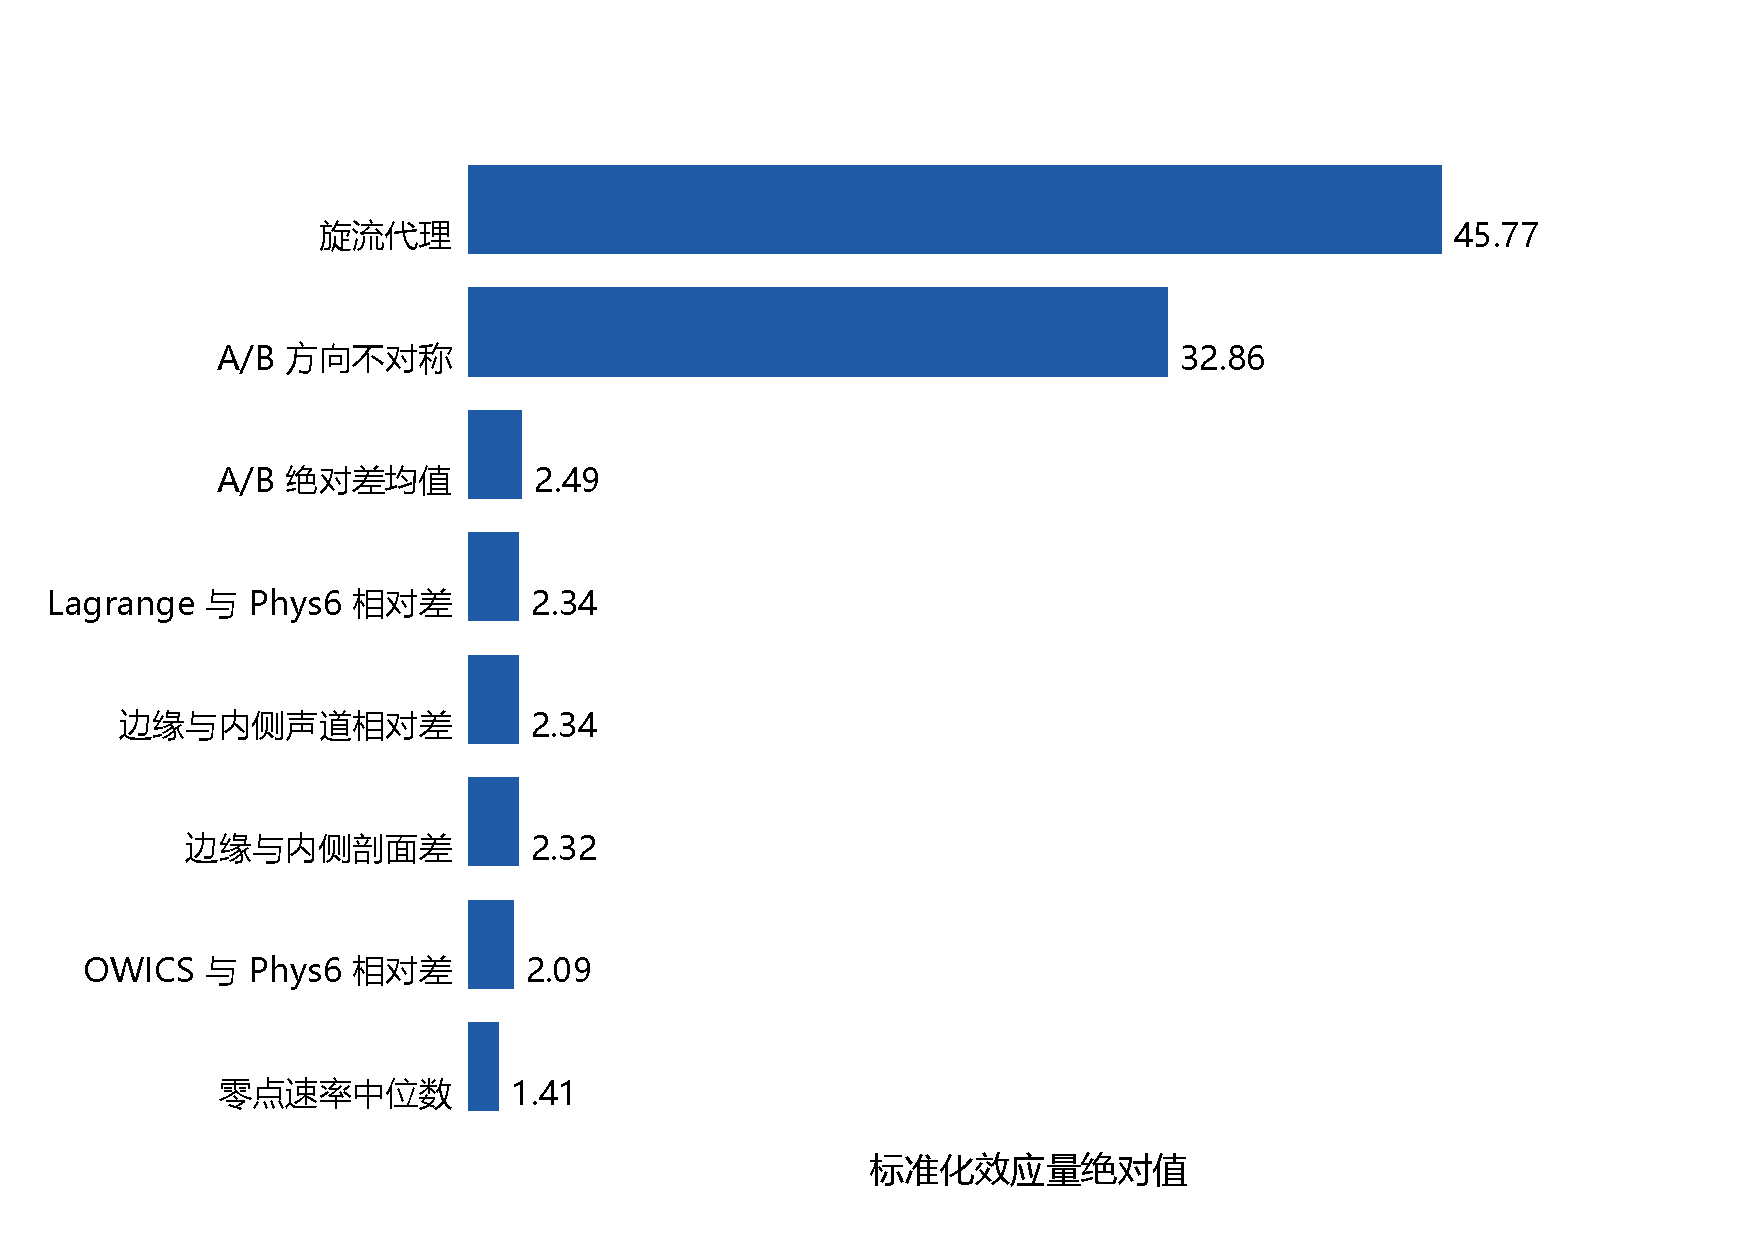
\includegraphics[width=0.88\textwidth]{../figures/fig_disturbance_feature_importance.pdf}
  \caption{扰流识别特征效应量排序}
  \label{fig:disturbance_feature_importance}
\end{figure}

\subsection{降维、聚类与失效机制}

PCA 只在 D1 至 D8 的扰流窗口上实施，输入为标准化后的紧凑物理特征。PC1 和 PC2 分别解释 $39.7544\%$ 与 $22.0094\%$ 的方差，二维累计解释率为 $61.7638\%$。加入第三个主成分后，该比例升至 $76.1964\%$；前五个主成分可覆盖 $90.1991\%$。

主要变化可以被少量主成分压缩，但二维图仍会丢失接近四成的信息。因此，图中的重叠不能简单解释成工况完全相同，分离现象也视高维结果综合判断。

\begin{figure}[!htbp]
  \centering
  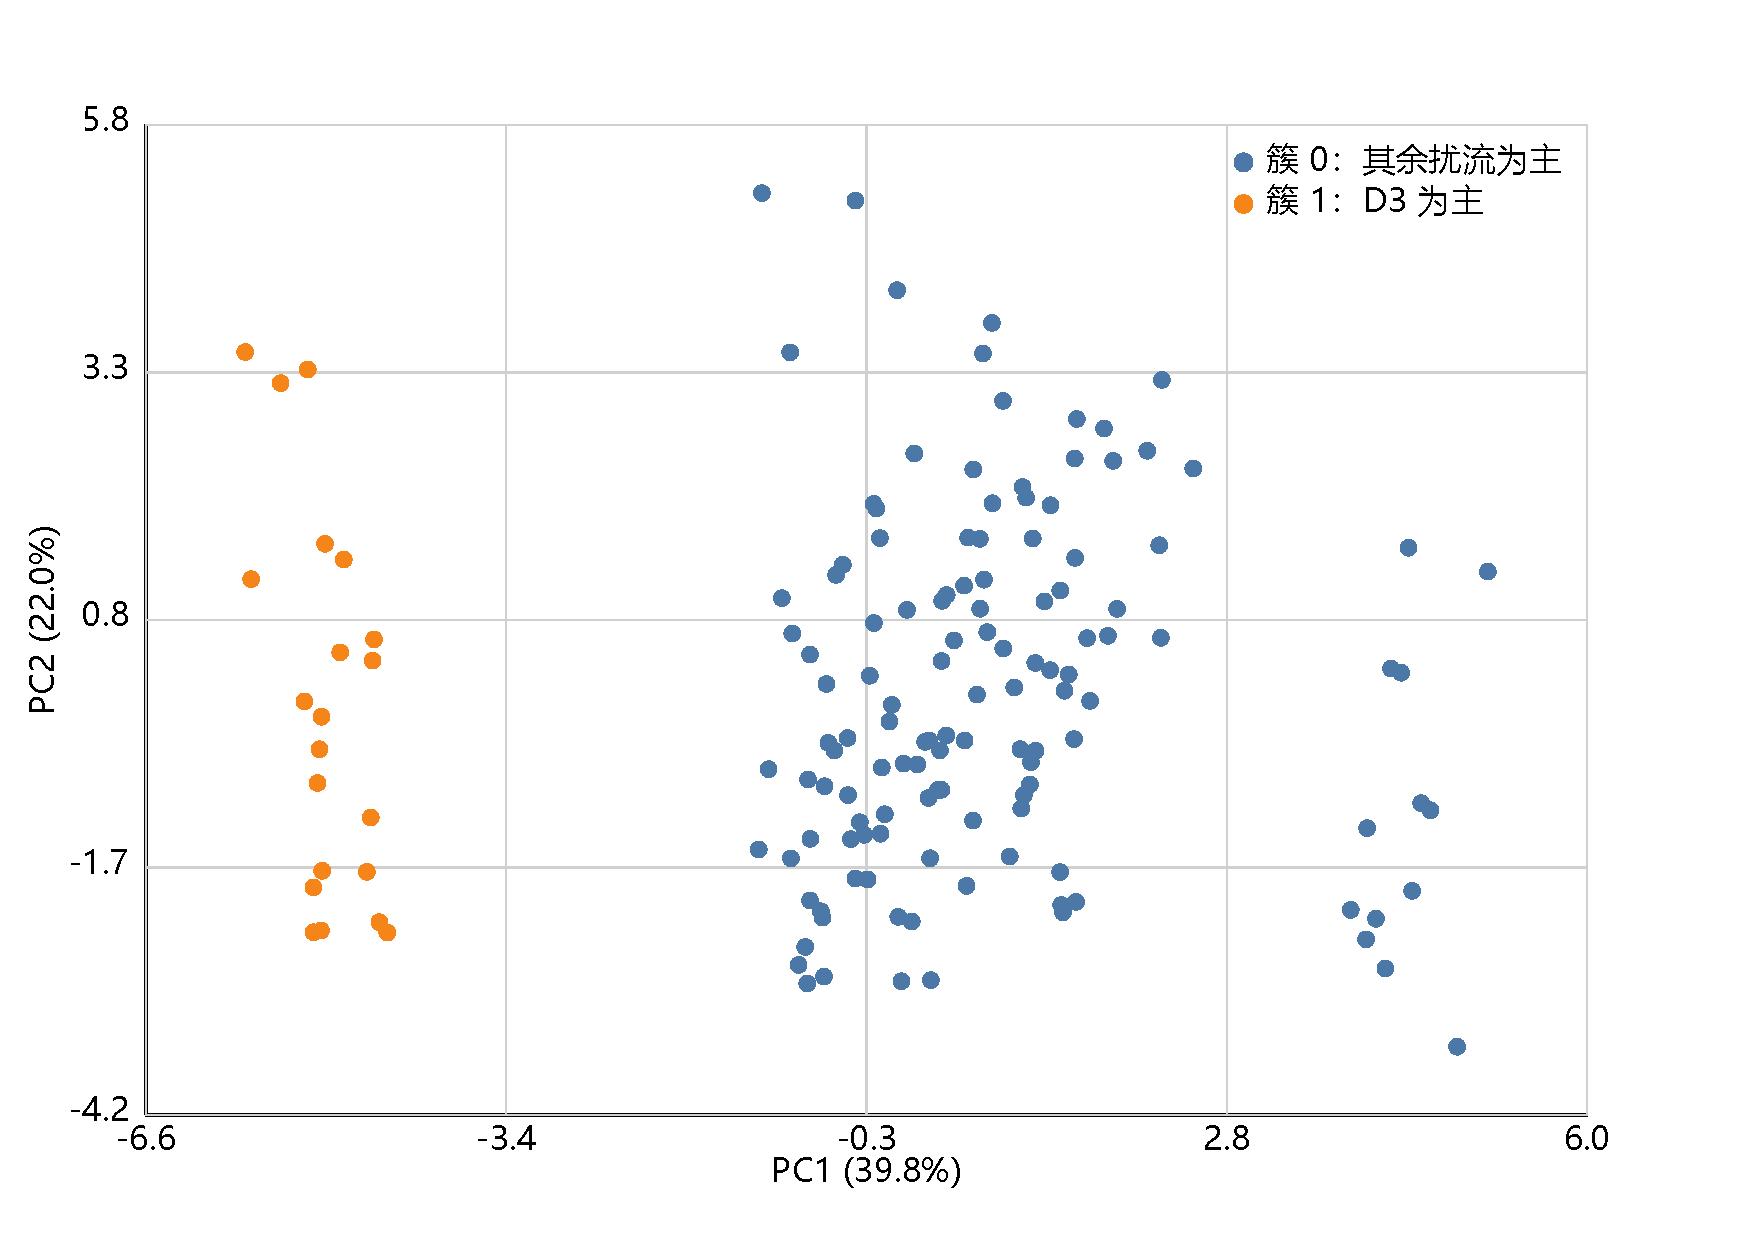
\includegraphics[width=0.86\textwidth]{../figures/fig_disturbance_pca_clusters.pdf}
  \caption{D1 至 D8 扰流窗口的 PCA 投影与最佳聚类}
  \label{fig:disturbance_pca}
\end{figure}

Qin 等曾用多声道观测训练 SVM，对 $65$ 种预设流型进行分类\cite{Qin2016ProfileIdentification}。说明多声道信息具备识别流型的潜力，但前提是类别边界清楚，训练样本也有足够覆盖。

本文分别运行 KMeans、Ward 层次聚类和对角 GMM，考察 $K=2,\ldots,5$。候选结果由 Silhouette、Calinski--Harabasz 与 Davies--Bouldin 指标共同评价。$K=2$ 的 KMeans 与 Ward 得到相同划分，三项指标均并列最优，分别为 $0.377676$、$56.9208$ 和 $0.98888$。后文采用 KMeans 标签展示交叉表。该轮廓系数只显示中等结构，并不支持强可分结论。

表~\ref{tab:cluster_disturbance_cross} 给出最佳聚类与人工扰流编号的交叉表。可以看到，一个簇几乎完全对应 D3，而 D1、D2、D4、D5、D6、D7、D8 大规模重叠在另一个簇中。这说明 \texttt{disturbance\_id} 更适合作为离线实验条件标签，而不能直接看作是在线流型类别。

\begin{table}[H]
\centering
\caption{最佳聚类与扰流编号交叉表}
\label{tab:cluster_disturbance_cross}
\begin{tabular}{ccccccccc}
\toprule
Cluster & D1 & D2 & D3 & D4 & D5 & D6 & D7 & D8 \\
\midrule
0 & 21 & 23 & 0 & 22 & 17 & 14 & 13 & 18 \\
1 & 0 & 0 & 21 & 0 & 0 & 0 & 0 & 0 \\
\bottomrule
\end{tabular}
\end{table}

把聚类标签与整组留出的失效诊断放在一起后，结论更为直接。系统漂移样本与重复性失稳样本混在同一簇中。D3 的位置相对独立，其他扰流编号却没有形成对应边界。若此时先做硬分类，再为每个簇训练独立补偿器，前一级的错分会继续传入流量估计。但是现有数据不足以支撑这条路线。

聚类未形成清晰类别，但不意味着特征无效。D1 至 D8 依然具有局部结构，只是整体更接近连续重叠分布。RBF 核可以按样本间距离平滑分配影响，因此比硬分类更贴合这种几何形态。软门控专家可在样本增加后作为局部增强尝试，由于样本数量限制当前仍以统一 KRR 为主。

综合来看，旋流代理、A/B 方向不对称、边缘--内侧差、中心--整体差和积分方法相对分歧能够表征扰流剖面变化；D3 相对独立，其余扰流状态高度重叠，无法形成稳定硬类别。因此，扰流编号只用于离线评价和机理解释，不作为在线输入。问题四将流量尺度与上述可观测剖面特征共同送入统一 RBF-KRR，使补偿随工况连续变化。
